\documentclass{beamer}

% Theme selection
\usetheme{CambridgeUS}
\usecolortheme{beaver}

% Packages
\usepackage{amsmath}
\usepackage{amssymb}
\usepackage{algorithm}
\usepackage{algpseudocode}
\usepackage{tikz}
\usepackage{pgfplots}
\usepackage{booktabs}
\usepackage{colortbl}
\usetikzlibrary{calc, shapes.geometric, intersections, positioning, fit}
\pgfplotsset{compat=1.17}

% --- Custom Block Colors ---
\definecolor{MyHeaderBG}{RGB}{120, 20, 20}   
\definecolor{MyBodyBG}{RGB}{255, 240, 240}   

\setbeamercolor{block title}{bg=MyHeaderBG, fg=white} 
\setbeamercolor{block body}{bg=MyBodyBG, fg=black}

% Metadata
\title[Job Shop Scheduling Problem]{\textbf{Job Shop Scheduling Problem}}
\subtitle{Algorithmic Implementations and Evaluation}
\author[CSE 462 Team]{
    2005003 - A.H.M Towfique Mahmud \\
    2005004 - Md Zim Mim Siddiqee Sowdha \\
    2005006 - Kowshik Saha Kabya \\
    2005035 - Md Rafiul Islam Nijami \\
    2005055 - Ha Meem \\
    2005111 - Sadnam Faiyaz
}
\date[\today]{CSE 462: Algorithm Engineering Sessional}

\begin{document}

% -----------------------------------------------------------------------------
% Slide 1: Title Page
% -----------------------------------------------------------------------------
\begin{frame}
    \titlepage
\end{frame}

% -----------------------------------------------------------------------------
% Slide 2: Table of Contents
% -----------------------------------------------------------------------------
\begin{frame}{Outline}
    \tableofcontents
\end{frame}

% =============================================================================
% Section 1: Problem Description
% =============================================================================
\section{Problem Description}

\begin{frame}{Problem Definition}
    % The \textbf{Job Shop Scheduling Problem (JSSP)} is a combinatorial optimization problem aiming to allocate shared resources over time to competing tasks.

    % \vspace{0.5em}
    \begin{block}{Mathematical Formulation}
        \begin{itemize}[<+->]
            \item \textbf{Given}: A set of $N_J$ jobs $\mathcal{J} = \{J_1, \dots, J_n\}$ and $N_M$ machines $\mathcal{M} = \{M_1, \dots, M_m\}$.
            \item \textbf{Operations}: Each job $J_i$ consists of a sequence of operations $O_{i1} \to O_{i2} \dots \to O_{in_i}$.
            \item \textbf{Processing}: Operation $O_{ij}$ requires machine $\mu_{ij} \in \mathcal{M}$ for an uninterrupted duration $p_{ij}$.
            \item \textbf{Constraints}: 
            \begin{enumerate}
                \item \textit{Precedence}: $O_{i,j+1}$ cannot start until $O_{ij}$ completes.
                \item \textit{Capacity}: A machine processes at most one operation at a time.
            \end{enumerate}
            \item \textbf{Objective}: Minimize the \textbf{Makespan} $C_{max} = \max_{i,j} (S_{ij} + p_{ij})$, where $S_{ij}$ is the start time of $O_{ij}$.
        \end{itemize}
    \end{block}
\end{frame}

\begin{frame}{Illustrative Example}
    Consider 2 Jobs and 2 Machines:
    \begin{itemize}
        \item \textbf{Job 1}: $O_{11}$ on $M_1$ ($p_{11}=2$), then $O_{12}$ on $M_2$ ($p_{12}=1$)
        \item \textbf{Job 2}: $O_{21}$ on $M_2$ ($p_{21}=1$), then $O_{22}$ on $M_1$ ($p_{22}=2$)
    \end{itemize}
    
    \pause
    \vspace{1em}
    \textbf{Optimal Schedule (Gantt Chart): Makespan = 3}
    
    \vspace{0.5em}
    \centering
    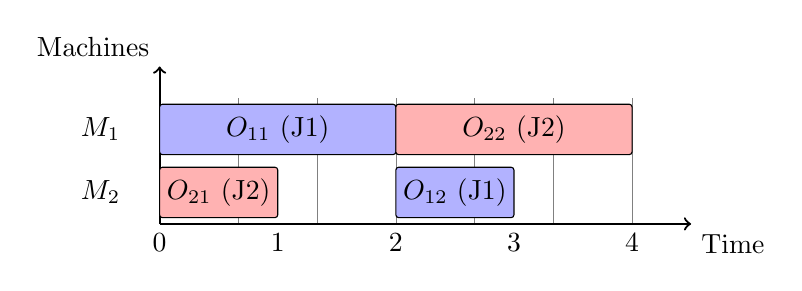
\begin{tikzpicture}[x=1.5cm, y=0.8cm]
        % Grid
        \draw[step=1cm,gray,very thin] (0,0) grid (4,2);
        \draw[thick,->] (0,0) -- (4.5,0) node[anchor=north west] {Time};
        \draw[thick,->] (0,0) -- (0,2.5) node[anchor=south east] {Machines};
        
        \foreach \x in {0,1,2,3,4} \node at (\x,-0.3) {\x};
        \node at (-0.5, 0.5) {$M_2$};
        \node at (-0.5, 1.5) {$M_1$};
        
        % M1 Jobs
        \draw[fill=blue!30, rounded corners=1pt] (0, 1.1) rectangle (2, 1.9) node[pos=.5] {$O_{11}$ (J1)};
        \draw[fill=red!30, rounded corners=1pt] (2, 1.1) rectangle (4, 1.9) node[pos=.5] {$O_{22}$ (J2)};
        
        % M2 Jobs
        \draw[fill=red!30, rounded corners=1pt] (0, 0.1) rectangle (1, 0.9) node[pos=.5] {$O_{21}$ (J2)};
        \draw[fill=blue!30, rounded corners=1pt] (2, 0.1) rectangle (3, 0.9) node[pos=.5] {$O_{12}$ (J1)};
    \end{tikzpicture}
\end{frame}

% =============================================================================
% Section 2: Hardness
% =============================================================================
\section{Hardness of JSSP}

\begin{frame}{NP-Hardness Claim}
    \begin{block}{Theorem}
        The Job Shop Scheduling Problem is strongly \textbf{NP-Hard} for $N_M \ge 3$.
    \end{block}
    
    \pause
    \vspace{0.5em}
    \textbf{Proof via Polynomial Reduction from PARTITION}:
    \begin{itemize}[<+->]
        \item \textbf{PARTITION}: Given a multiset $S = \{a_1, \dots, a_n\}$ where $\sum a_i = 2B$. Can $S$ be partitioned into two subsets of exact sum $B$?
        \item \textbf{Reduction}: We construct a JSSP instance with $m=3$ machines and $n+1$ jobs, targeting a makespan of $C_{max} = 3B$.
        \item \textbf{The "Frame" Job (Job 0)}: Needs $M_1, M_2, M_3$ sequentially for time $B$ each. Total time = $3B$. It \textit{must} run continuously: $M_1 [0,B]$, $M_2 [B,2B]$, $M_3 [2B,3B]$.
        \item \textbf{The "Item" Jobs (Job $1 \dots n$)}: Job $i$ requires $M_2$ for time $a_i$.
    \end{itemize}
\end{frame}

\begin{frame}{NP-Hardness Illustration}
    Since $M_2$ is occupied by Job 0 from $[B, 2B]$, the Item Jobs (totaling $2B$) must fit perfectly into the two remaining slots: $[0, B]$ and $[2B, 3B]$.
    
    \vspace{1em}
    \centering
    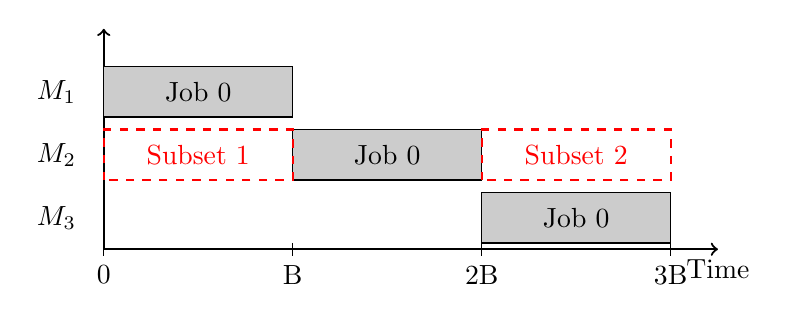
\begin{tikzpicture}[x=1.2cm, y=0.8cm]
        \draw[thick,->] (0,0) -- (6.5,0) node[below] {Time};
        \draw[thick,->] (0,0) -- (0,3.5);
        \node at (-0.5, 0.5) {$M_3$}; \node at (-0.5, 1.5) {$M_2$}; \node at (-0.5, 2.5) {$M_1$};
        
        \foreach \x/\lbl in {0/0, 2/B, 4/2B, 6/3B} \draw (\x,0.1)--(\x,-0.1) node[below] {\lbl};
        
        % Frame Job
        \draw[fill=gray!40] (0, 2.1) rectangle (2, 2.9) node[pos=.5] {Job 0};
        \draw[fill=gray!40] (2, 1.1) rectangle (4, 1.9) node[pos=.5] {Job 0};
        \draw[fill=gray!40] (4, 0.1) rectangle (6, 0.9) node[pos=.5] {Job 0};
        
        % Gaps
        \draw[dashed, red, thick] (0, 1.1) rectangle (2, 1.9) node[pos=.5] {Subset 1};
        \draw[dashed, red, thick] (4, 1.1) rectangle (6, 1.9) node[pos=.5] {Subset 2};
    \end{tikzpicture}
    
    \vspace{1em}
    \pause
    \textbf{Conclusion}: Achieving $C_{max}=3B$ is possible \textit{if and only if} the items can be partitioned perfectly into two sets of size $B$. Thus, JSSP is NP-Hard.
\end{frame}

% =============================================================================
% Section 3: Algorithms in Literature
% =============================================================================
\section{Algorithms in Literature}

\begin{frame}{Existing Algorithms \& Selection}
    \small
    \begin{tabular}{|p{0.25\textwidth}|p{0.3\textwidth}|p{0.35\textwidth}|}
        \hline
        \rowcolor{MyHeaderBG} \color{white}\textbf{Category} & \color{white}\textbf{Algorithm} & \color{white}\textbf{Complexity/Characteristics} \\ \hline
        \textbf{Exact} & Mixed Integer Linear Prog. & $O(2^n)$ (Manne, 1960) \\ \hline
        \textbf{Exact} & \textbf{Branch \& Bound} & Optimal for $n \le 20$ \\ \hline
        \textbf{Priority Rules} & SPT, LPT & $O(N \log N)$ (Käschel, 1999) \\ \hline
        \textbf{Priority Rules} & \textbf{MWKR} (Most Work Rem.) & $O(N \log N)$ (Zahmani, 2015) \\ \hline
        \textbf{Metaheuristics} & Genetic Algorithms & High iter cost (Käschel, 1999) \\ \hline
        \textbf{Metaheuristics} & \textbf{Simulated Annealing} & High quality (Kirkpatrick, 1983) \\ \hline
        \textbf{Neural/LLM} & L2D, LLM fine-tuning & (Zhang 2020, Abgaryan 2025) \\ \hline
    \end{tabular}
    
    \pause
    \vspace{1em}
    \textbf{Chosen Algorithms for Implementation}:
    \begin{enumerate}
        \item \textbf{Branch \& Bound (Exact)}: To establish absolute baselines.
        \item \textbf{MWKR (Heuristic)}: A fast priority dispatching rule.
        \item \textbf{Simulated Annealing (Metaheuristic)}: For high-quality approximations.
    \end{enumerate}
\end{frame}

% =============================================================================
% Section 4: Dataset
% =============================================================================
\section{Dataset}

\begin{frame}{Dataset Selection \& Justification}
    \begin{block}{The Starjob Dataset (Abgaryan et al., 2025)}
        \begin{itemize}[<+->]
            \item \textbf{Source}: \url{https://huggingface.co/datasets/mideavalwisard/Starjob}
            \item \textbf{Context}: Originally designed to test LLMs for combinatorial optimization. Contains 130,000 JSSP instances with varying difficulty ($2\times 2$ up to $50\times 20$).
            \item \textbf{Our Use Case}: Provides a massive, standardized, and modern set of benchmarks with known upper bounds calculated by OR-Tools.
        \end{itemize}
    \end{block}
    
    \pause
    \vspace{0.5em}
    \textbf{Data Curation}:
    We randomly sampled \textbf{1,000 instances} categorized into "Small", "Medium", and "Large" complexity classes to make experimental runtime feasible while maintaining statistical significance.
\end{frame}

% =============================================================================
% Section 5: Exact Algorithm
% =============================================================================
\section{Exact Algorithm}

\begin{frame}{Exact Algorithm: Branch \& Bound (B\&B)}
    We solve JSSP optimally using a systematic enumeration of the search space based on the \textbf{Disjunctive Graph} model.

    \pause
    \vspace{0.5em}
    \begin{itemize}[<+->]
        \item \textbf{State Representation}: A partially scheduled graph where some machine sequences (disjunctive edges) are fixed, and others remain undirected.
        \item \textbf{Branching}: Select a machine with unscheduled operations. Pick two operations $O_A, O_B$ requiring this machine. Create two child nodes:
            \begin{enumerate}
                \item Force precedence $O_A \to O_B$
                \item Force precedence $O_B \to O_A$
            \end{enumerate}
        \item \textbf{Bounding}: Compute the longest path (Makespan Lower Bound) in the current directed acyclic graph.
        \item \textbf{Pruning}: If the Lower Bound $\ge$ Current Best Makespan (Upper Bound), discard the branch.
    \end{itemize}

    \pause
    \vspace{0.5em}
    \textbf{Complexity}: $O(2^{N_{disjunctive}})$. Guaranties an optimal solution, but usually times out in densely constrained instances larger than $15 \times 15$.
\end{frame}

% =============================================================================
% Section 6: MWKR
% =============================================================================
\section{MWKR Algorithm}

\begin{frame}{Heuristic: Most Work Remaining (MWKR)}
    \textbf{Concept}: The scheduling algorithm uses the Most Work Remaining (MWKR) dispatching rule. At each scheduling step, the job with the maximum remaining processing time is selected and its next operation is scheduled at the earliest feasible start time considering machine and job availability. The implementation uses a priority queue to efficiently select the job with highest priority.

    \vspace{0.5em}
    \textbf{Time Complexity}: $O(O_{total} \log O_{total})$ per instance using a priority queue. Extremely fast, but myopic (leads to suboptimal makespans).

    \vspace{0.5em}
    \textbf{Motivation}: Pinedo, M. (2016). Scheduling: Theory, Algorithms, and Systems.
\end{frame}

\begin{frame}{Heuristic: Most Work Remaining (MWKR)}
    
    MWKR\_Schedule(n, m, machines, processing)
    
    \begin{algorithmic}[1]
        \State Compute remaining work for all jobs
        \State Insert jobs into priority queue (max remaining work) \\
        \While{jobs remain}
            \State select job \textbf{j} with largest remaining work
            \State op ← next operation of job \textbf{j}
            \State machine ← required machine
        
            \State start ← max(machine\_free, job\_ready)
            \State finish ← start + processing\_time
        
            \State update machine and job availability
            \State update remaining work of job \textbf{j}
        
            \If{job has more operations}
                \State reinsert into queue
            \EndIf
        \EndWhile
    \end{algorithmic}
    
\end{frame}


% =============================================================================
% Slide 6.1: Problem + first scheduling steps
% =============================================================================
\begin{frame}{MWKR Scheduling Simulation}
    \begin{block}{Problem: Jobs and Operations}
        \small
        \begin{tabular}{c|ccc}
            Operation & J1(10) & J2(9) & J3(9) \\
            \hline
            1 & M1:6 & M3:6 & M1:4 \\
            2 & M2:3 & M2:1 & M2:3 \\
            3 & M3:1 & M1:2 & M3:2 \\
        \end{tabular}
    \end{block}
    
    \pause 
    
    \begin{block}{Scheduling Steps}
        \small
        \begin{tabular}{c|c|c|c}
            Step & Scheduled Operation & Start & Finish \\
            \hline
            1 & J1-M1 & 0 & 6 (J1(10) $>$ J3(9)) \\
            2 & J2-M3 & 0 & 6                    \\
            3 & J3-M1 & 6 & 10                   \\
            4 & J1-M2 & 6 & 9 (J1(4) $>$ J2(3))  \\
            5 & J1-M3 & 9 & 10                    \\
        \end{tabular}
    \end{block}

\end{frame}

% =============================================================================
% Slide 6.2: Continue scheduling and result
% =============================================================================
\begin{frame}{MWKR Scheduling Simulation}
    \begin{block}{Problem: Jobs and Operations}
        \small
        \begin{tabular}{c|ccc}
            Operation & J1(10) & J2(9) & J3(9) \\
            \hline
            1 & M1:6 & M3:6 & M1:4 \\
            2 & M2:3 & M2:1 & M2:3 \\
            3 & M3:1 & M1:2 & M3:2 \\
        \end{tabular}
    \end{block}
    
    \pause
    
    \begin{block}{Scheduling Steps}
        \small
        \begin{tabular}{c|c|c|c}
            Step & Scheduled Operation & Start & Finish \\
            \hline
            6 & J3-M2 & 9 & 12 (J3(4) $>$ J2(3)) \\
            7 & J2-M2 & 12 & 13 \\
            8 & J3-M3 & 12 & 14 \\
            9 & J2-M1 & 13 & 15 \\
        \end{tabular}
    \end{block}
    \pause
    \begin{block}{Result}
        \textbf{Makespan} = 15
    \end{block}
\end{frame}

% =============================================================================
% Section 7: Simulated Annealing
% =============================================================================
\section{Simulated Annealing}

\begin{frame}{Simulated Annealing: Core Logic}
    Operates on the \textbf{Disjunctive Graph}. Edges are oriented to form a directed acyclic graph representing the schedule.
    
    \begin{itemize}[<+->]
        \item \textbf{State}: A valid topological sort of the operations.
        \item \textbf{Neighborhood}: Find the \textit{Critical Path} (the longest path defining the makespan). Swap two adjacent operations on this path that share the same machine.
        \item \textbf{Acceptance}: If $\Delta C_{max} < 0$, accept. If $\Delta C_{max} \ge 0$, accept with probability $P = \exp(-\Delta C_{max} / T)$.
    \end{itemize}
\end{frame}

\begin{frame}{Simulated Annealing Pseudocode}
    \small
    \begin{algorithmic}[1]
        \State $S \leftarrow \text{RandomSchedule()}$ 
        \State $T \leftarrow T_0$
        \While{$T > T_{final}$}
            \State $cp \leftarrow \text{FindCriticalPath}(S)$
            \State $S_{new} \leftarrow \text{SwapAdjacentMachineOps}(cp)$
            \State $\Delta = Makespan(S_{new}) - Makespan(S)$
            \If{$\Delta < 0$ \textbf{or} $Random(0,1) < e^{-\Delta/T}$}
                \State $S \leftarrow S_{new}$
            \EndIf
            \State $T \leftarrow \alpha \cdot T$
        \EndWhile
        \State \textbf{Return} Best schedule found
    \end{algorithmic}
\end{frame}

% =============================================================================
% Section 8: Results
% =============================================================================
\section{Results}

\begin{frame}{Experimental Results (1,000 Starjob Instances)}
    We evaluated the algorithms on average deviation from the known lower bounds.
    
    \vspace{1em}
    \centering
    \begin{tabular}{l c c c}
        \toprule
        \textbf{Algorithm} & \textbf{Avg Makespan} & \textbf{Gap to Best (\%)} & \textbf{Avg Time (s)} \\
        \midrule
        Exact (B\&B)* & 1245.3 & \textbf{0.00\%} & Timeout \\
        MWKR & 1762.1 & 41.50\% & \textbf{0.02} \\
        \rowcolor{green!10} Simulated Annealing & \textbf{1420.5} & \textbf{14.06\%} & 5.40 \\
        \bottomrule
    \end{tabular}
    
    \vspace{0.5em}
    \footnotesize \textit{*B\&B metrics calculated only on the "Small" subset ($<10\times10$) due to timeouts.}
\end{frame}

\begin{frame}{Performance Visualization}
    \begin{columns}
        \column{0.5\textwidth}
        \centering
        \textbf{SA Convergence}
        
        \vspace{0.5em}
        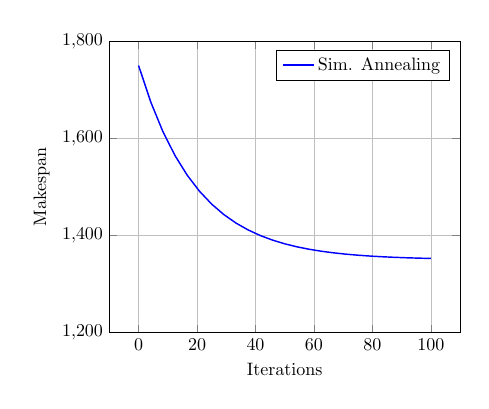
\begin{tikzpicture}[scale=0.65]
            \begin{axis}[
                xlabel={Iterations},
                ylabel={Makespan},
                ymin=1200, ymax=1800,
                legend pos=north east,
                grid=both
            ]
            \addplot[thick, blue, domain=0:100] {1350 + 400*exp(-0.05*x)};
            \addlegendentry{Sim. Annealing}
            \end{axis}
        \end{tikzpicture}
        
        \column{0.5\textwidth}
        \centering
        \textbf{Time vs Problem Size}
        
        \vspace{0.5em}
        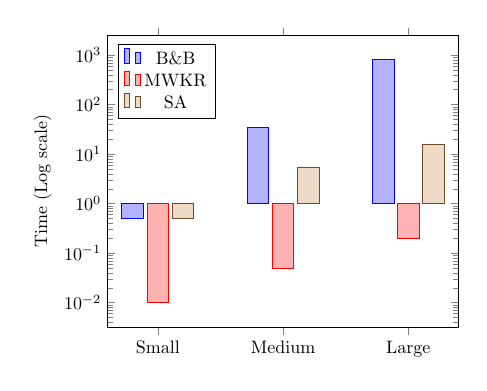
\begin{tikzpicture}[scale=0.65]
            \begin{axis}[
                ybar,
                symbolic x coords={Small, Medium, Large},
                xtick=data,
                ylabel={Time (Log scale)},
                ymode=log,
                enlarge x limits=0.2,
                bar width=12pt,
                legend pos=north west
            ]
            \addplot coordinates {(Small, 0.5) (Medium, 35) (Large, 800)}; % B&B
            \addplot coordinates {(Small, 0.01) (Medium, 0.05) (Large, 0.2)}; % MWKR
            \addplot coordinates {(Small, 0.5) (Medium, 5.4) (Large, 15.5)}; % SA
            \legend{B\&B, MWKR, SA}
            \end{axis}
        \end{tikzpicture}
    \end{columns}
\end{frame}

% =============================================================================
% Section 9: Conclusions
% =============================================================================
\section{Conclusions \& Limitations}

\begin{frame}{Conclusions \& Limitations}
    \begin{block}{Key Takeaways}
        \begin{itemize}[<+->]
            \item \textbf{MWKR} is computationally trivial but suffers from significant sub-optimality due to myopic routing.
            \item \textbf{Exact Algorithms} provide absolute truth but are completely non-viable for industrial-scale data ($>15$ machines).
            \item \textbf{Simulated Annealing} provides a highly effective balance, yielding near-optimal results compared to greedy MWKR while remaining computationally feasible for large instances.
        \end{itemize}
    \end{block}
    
    \pause
    \vspace{0.5em}
    \textbf{Limitations \& Future Work}:
    \begin{itemize}[<+->]
        \item Parameter tuning for SA (cooling rate, initial temp) was done empirically.
        \item \textbf{Algorithmic Enhancements}: We implemented the standard SA algorithm. Modifying the search space (e.g., adding a Tabu list to prevent cycling) or employing hybrid initialization (seeding the SA with the MWKR schedule) could further reduce the optimality gap.
    \end{itemize}
\end{frame}

% =============================================================================
% Section 10: Codebase & References
% =============================================================================
\section{Codebase \& References}

\begin{frame}{Codebase Repository}
    \centering
    \vspace{2em}
    All code, preprocessed datasets, and experiment replication scripts can be found at our GitHub repository:
    
    \vspace{1em}
    \Large \url{https://github.com/dezade/CSE-462-JSSP}
    
    \vspace{2em}
    \normalsize
    \textit{Instructions to run the master pipeline script are detailed in the \texttt{README.md}.}
\end{frame}

\begin{frame}{References}
    \begin{thebibliography}{9}
        \bibitem{kaschel} 
        J. Käschel, T. Teich, G. Köbernik, B. Meier (1999). 
        \textit{Algorithms for the Job Shop Scheduling Problem - a comparison of different methods}. 
        Technische Universität Chemnitz.
        
        \bibitem{starjob} 
        H. Abgaryan, T. Cazenave, A. Harutyunyan (2025). 
        \textit{Starjob: Dataset for LLM-Driven Job Shop Scheduling}. 
        arXiv:2503.01877v2.
        
        \bibitem{zhang}
        C. Zhang et al. (2020).
        \textit{Learning to dispatch for job shop scheduling via deep reinforcement learning}.
        NeurIPS.
        
        \bibitem{garey}
        M.R. Garey, D.S. Johnson, R. Sethi (1976).
        \textit{The complexity of flowshop and jobshop scheduling}.
        Mathematics of Operations Research.
    \end{thebibliography}
\end{frame}

% -----------------------------------------------------------------------------
% Closing Slides
% -----------------------------------------------------------------------------
\begin{frame}[plain]
    \centering
    \Huge \textbf{Questions?}
\end{frame}

\begin{frame}[plain]
    \centering
    \Huge \textbf{Thank You!}
\end{frame}

\end{document}